\documentclass[aspectratio=169]{beamer}
\mode<presentation>
%\usetheme{Warsaw}
%\usetheme{Goettingen}
\usetheme{Hannover}
%\useoutertheme{default}

%\useoutertheme{infolines}
\useoutertheme{sidebar}
\usecolortheme{dolphin}


\setbeamersize{sidebar width left=0pt} % to remove the sidebar
\beamertemplatenavigationsymbolsempty % To remove the navigation symbols on the bottom right.
\setbeamersize{text margin left=10mm,text margin right=10mm} % Specify margins

\usepackage{amsmath}
\usepackage{amssymb}
\usepackage{listings}
\usepackage{enumerate}
\usepackage{hyperref}
\hypersetup{
    colorlinks=true,
    linkcolor=blue,
    filecolor=magenta,      
    urlcolor=cyan,
}
 
\urlstyle{same}

%some bold math symbosl
\newcommand{\Cov}{\mathrm{Cov}}
\newcommand{\Var}{\mathrm{Var}}
\newcommand{\brho}{\boldsymbol{\rho}}
\newcommand{\bSigma}{\boldsymbol{\Sigma}}
\newcommand{\btheta}{\boldsymbol{\theta}}
\newcommand{\bbeta}{\boldsymbol{\beta}}
\newcommand{\bmu}{\boldsymbol{\mu}}
\newcommand{\bW}{\mathbf{W}}
\newcommand{\one}{\mathbf{1}}
\newcommand{\bH}{\mathbf{H}}
\newcommand{\by}{\mathbf{y}}
\newcommand{\bolde}{\mathbf{e}}
\newcommand{\bx}{\mathbf{x}}

\newcommand{\cpp}[1]{\texttt{#1}}

%--------------------------------------------------
\providecommand{\abs}[1]{\lvert#1\rvert}
\providecommand{\norm}[1]{\lVert#1\rVert}
\providecommand{\Blue}[1]{\textcolor{blue}{#1}}
\providecommand{\Red}[1]{\textcolor{red}{#1}}
\newcommand{\celsius}{\ensuremath{^\circ}C}
\newcommand\thfore{\mathord{\therefore}\,}
%------------------------------------------------------------------

\title{Lecture 20. Recurrence Relations}
%\author{\includegraphics[width=.5\textwidth,height=.5\textheight]{lecture4-fig0.png}}

\date{ }
%------------------------------------------------------------------


\begin{document}

\frame[plain]{\titlepage}

\begin{frame}[plain]{Recurrence Relations (or Recursion)}

  Suppose we want to define a function
    $ P: \mathbb{N}\rightarrow\mathbb{Z}$  
    \begin{enumerate}
      \item The easiest way is to give 
      an \Blue{explicit} formula~\footnote{also, called 
        \Blue{a closed formula} or \Blue{closed-form solution to a recurrence
        relation}}:
        \[ P(n)= \frac{n(n+1)}{2}  \] 
      \item Another way is to \Blue{define recursively}
        \[ P(n) = \left\{  \begin{array}{ccc}
                            1 &\mbox{if}& n=1\\
                            n+P(n-1) &\mbox{if}& n>1.
                           \end{array} \right. 
        \]
        This is a \Blue{recurrence relation}; that is,  $P(n)$ 
        expressed
        in terms of one or more of the previous terms of the rule, namely, 
        $P(0), P(1), ..., P(n-1)$. 
        
    \end{enumerate} 

\end{frame}

\begin{frame}[plain]{Three Laws of Recursion}

   A \Red{well-defined} recurrence relation (recursion) obeys three important laws:
    \begin{enumerate}
      \item A recursion must have a nonrecursive 
           \Blue{base case} that gives at least one value of the function explicitly.  
     \item A recursion must call itself, repeatedly.
      \item A recursion must change its state and move toward the base case.
    \end{enumerate}
    \medskip
    
   For example, 
    \[ P(n) = \left\{  \begin{array}{ccc}
                            1 &\mbox{if}& n=1\\
                            n+P(n-1) &\mbox{if}& n>1.
                           \end{array} \right. 
        \]
        satisfies all three laws.
 
\end{frame}

\begin{frame}[plain]{}


 {\bf Example 20.1}.   
   Find a recurrence relation $P(n)$ that yields the following sequence:
     \[ 5, 11, 18, 26, 35, 45, ... \] %Essential, sec 3.1, p162, 19(b)\\
   Then, find the closed formula for $P(n)$.   
   
   \pause
   
   \begin{itemize}
    \item Answer:
      \begin{align*}
       P(n) &= \left\{  \begin{array}{ccc}
                            5 &\mbox{if}& n=0\\
                            P(n-1)+5+n &\mbox{if}& n\geq 1
                           \end{array} \right.  \\
            P(n) &= 5+5n+\frac{n(n+1)}{2} \ \ \mbox{for}\ n=0,1,2,...                                                       
      \end{align*}  
   \end{itemize}
   
 
   
  \vspace{.7in}
  
\end{frame}

\begin{frame}[plain]{}

  {\bf Practice 20.2}%~\footnote{
 % Sum of Arithmetic Sequence = $\frac{n}{2}\{ 2a_0+(n-1)d\}$
 % }
\ \      Find a recursive definition and 
 an explicit formula
  for the sequence below. Assume the first term listed is $a_0$:
   \[ 50, 43, 36, 29, .... \]
   %https://discrete.openmathbooks.org/dmoi2/sec_seq-arithgeom.html
   
   \pause
   
   \begin{itemize}
    \item Answer:
      \begin{align*}
       A(n) &= \left\{  \begin{array}{ccc}
                            50 &\mbox{if}& n=0\\
                            A(n-1)-7 &\mbox{if}& n\geq 1
                           \end{array} \right.  \\
            A(n) &= 50 - 7n \ \mbox{for}\ n=0,1,2,...                            
      \end{align*}  
   \end{itemize}
   
  \vspace{.7in}
  
\end{frame}

\begin{frame}[plain]{The Fibonacci Sequence}
 \begin{itemize}
  \item In the early thirteenth century, the Italian mathematician Leonardo Pisano Fibonacci
     proposed the following problem. 
    \begin{columns}[c]
      \column{.5\textwidth}
         A certain person put {\bf a pair of rabbits} in a place surrounded by
          a wall.
          \medskip
          
          If \Blue{every month} each pair begets a new pair \Red{from the second month}, 
          how many pairs of rabbits can be produced from that pair in a year?
          
      \column{.5\textwidth} 
	\begin{center}
	      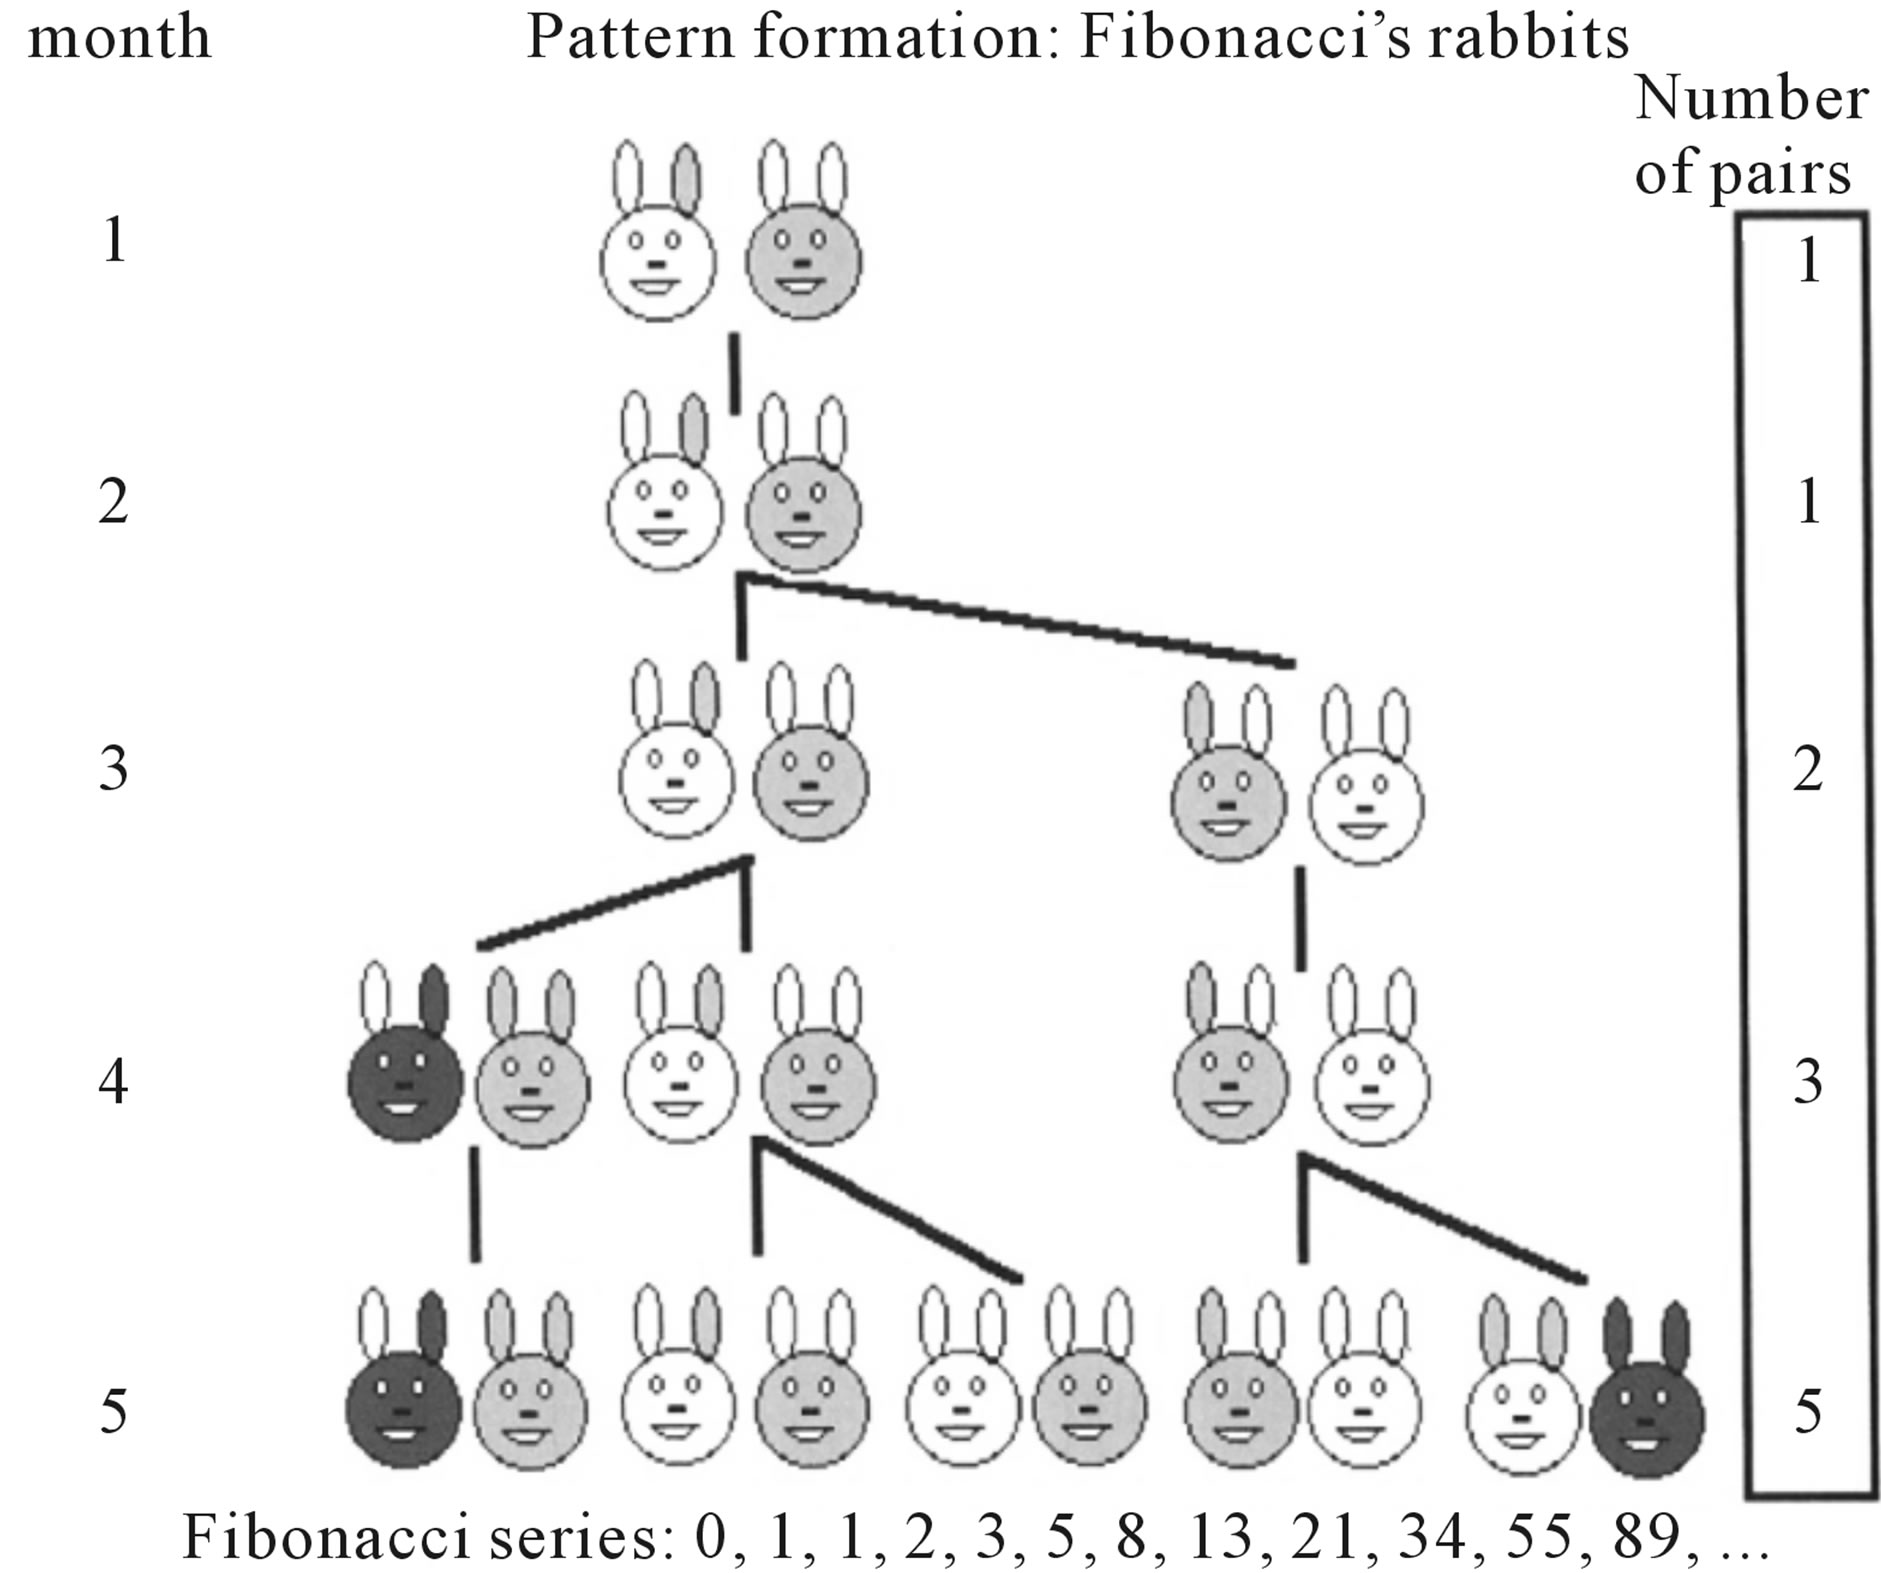
\includegraphics[height=5.5cm]{./img/lecture20-fig1.jpg}
	  \end{center}  
   \end{columns}
     
 \end{itemize}

\end{frame}

\begin{frame}[plain]{ }
 
   The \Blue{Fibonacci numbers} $F(n)$ satisfy the following recurrence relation:
     \[ \Blue{
          F(n) = \left\{ \begin{array}{ccc}
                          1 &\mbox{if}& n=1\ \mbox{or}\ n=2\\
                          F(n-1)+F(n-2)&\mbox{if}& n>2.
                         \end{array}
                  \right. 
              }
     \]
  
   {\bf Example 20.3}. Use the above function to list the Fibonacci numbers.
   \pause
   \medskip
   
    The \Blue{Fibonacci numbers:} 1, 1, 2, 3, 5, 8, 13, 21, 34, 55, 89, ...
   \medskip
  
	\begin{center}
	         Recursive Implementation of Fibonacci numbers in Python
	         
	      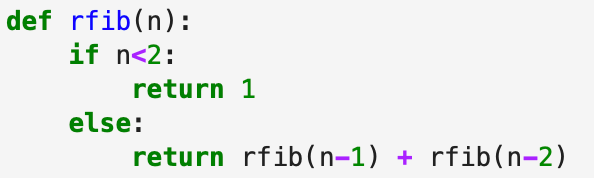
\includegraphics[height=2cm]{./img/lecture20-fig2.png}
	  \end{center}  


 
%  \vspace{1.2in}
  
\end{frame}


%%%%%%%%%%%%%%%%%%%
\iffalse

\begin{frame}[plain]{The Fibonacci Sequence\footnote{Source: 
  http://www.3villagecsd.k12.ny.us/wmhs/Departments/Math/OBrien/fibonacci2.html}
   }
 \begin{itemize}
   \item  The \Blue{Fibonacci numbers:} 1, 1, 2, 3, 5, 8, 13, 21, 34, 55, 89, ...
  \item Here you see that there are, for example, 8 or 13 {\bf whirls on a pinecone} 
    (both fibonacci numbers) depending on which direction you follow. If you also look at 
  a pinecone from the side, each level has a certain number of scales that matches a Fibonacci number.
    \begin{columns}[c]
      \column{.4\textwidth}
        \begin{center}
	      \includegraphics[height=4.5cm]{lecture23-fig2.jpg}
	  \end{center} 
      \column{.4\textwidth} 
	\begin{center}
	      \includegraphics[height=4.5cm]{lecture23-fig3.jpg}
	  \end{center}  
   \end{columns}
 \end{itemize}

\end{frame}

\begin{frame}[plain]{The Fibonacci Sequence\footnote{Source: 
  http://www.3villagecsd.k12.ny.us/wmhs/Departments/Math/OBrien/fibonacci2.html}}
 \begin{itemize}
   \item  The \Blue{Fibonacci numbers:} 1, 1, 2, 3, 5, 8, 13, 21, 34, 55, 89, ...
  \item Pinecones are not alone. Just about every plant or animal is governed by 
    Fibonacci numbers! Here's another example.
    \begin{columns}[c]
      \column{.4\textwidth}
        You can tell how the leaves of the plant (8, another Fibonacci number) go up in spirals so that 
      from the top view, we can see that 
      {\bf each leaf gets as much sunlight as possible}. The spirals themselves are 
      in Fibonacci increments and proportions.
      \column{.4\textwidth} 
	\begin{center}
	      \includegraphics[height=4cm]{lecture23-fig4.jpg}
	  \end{center}  
   \end{columns}
   \item Other examples at 
   http://www.quora.com/What-are-the-real-life-applications-of-Fibonacci-series
 \end{itemize}

\end{frame}

\fi
%%%%%%%%%%%%%%%%%

%%\begin{frame}[plain]{Fibonacci Retracements and Fibonacci Ratios }
 %%  One of the remarkable characteristics of this Fibonacci's sequence 
 %%      is that each number is approximately 1.618 times greater than the preceding number. 
  %%     This common relationship between every number in the series is the foundation of 
  %%     the ratios used by technical traders to determine retracement levels.

  
 %%  \begin{itemize}
  %%   \item \Blue{Fibonacci retracements} are popular tools that traders can use to draw support lines, 
 %%     identify resistance levels, place stop-loss orders, and set target prices.
  %%   \item A Fibonacci retracement is created by taking two extreme points on a stock chart 
  %%   and dividing the vertical distance by the key Fibonacci ratios of
  %%   23.6\%, 38.2\%, 50\%, 61.8\%, and 100\%.
   %%  \item For example,    
   %%    The key Fibonacci ratio of 61.8\% is found by dividing one number in the series 
   %%    by the number that follows it. For example, 21 divided by 34 equals 0.6176, 
 %%      and 55 divided by 89 equals about 0.61798.
 %% \end{itemize}
 
 %% For more explanations, check this website: 
 %% \href{https://www.investopedia.com/ask/answers/05/fibonacciretracement.asp#:~:text=Fibonacci\%20retracements\%20are\%20popular\%20among\%20technical\%20traders.&text=In\%20technical\%20analysis\%2C\%20a\%20Fibonacci,61.8\%25\%2C\%20and\%20100\%25.}{How Fibonacci Ratios Work}~\footnote{
 %%\tiny{ 
%%   \url{https://www.investopedia.com/ask/answers/05/fibonacciretracement.asp#:~:text=Fibonacci\%20retracements\%20are\%20popular\%20among\%20technical\%20traders.&text=In\%20technical\%20analysis\%2C\%20a\%20Fibonacci,61.8\%25\%2C\%20and\%20100\%25} }
 %%  }
%%\end{frame}

\begin{frame}[plain]{}

  {\bf Practice 20.4}.  Suppose we model the spread of a virus in a certain population as follows.
  On day 1, one person is infected. On each subsequent day, each infected person gives the cold 
  to two others.
    \begin{itemize}
      \item[(a)] Write down a recurrence relation for this model.
      \item[(b)] What are some of the limitations of this model? How does it fail to be realistic?
    \end{itemize}
 \pause 
 
 \medskip
 
 Answer: The recurrence relation $V(n)$ for the number of infected persons is 
    \[ V(n) = \left\{ \begin{array}{ccc}
                       1 &\mbox{if}& n=1\\
                       V(n-1)+ 2V(n-1)&\mbox{if} & n>1
                      \end{array}\right. 
     \]       
     There are several unrealistic aspects: For example, nobody ever gets better, and there is no limit on the %number of people 
     who get infected, etc.      
        
     \vspace{.5in}
     
 \end{frame}
 
 
\begin{frame}[plain]{}

  {\bf Example 20.5}. 
  Suppose that you are collecting coins to make hexagons in a natural way
    by packing circles as tightly as possible.
    \begin{center}
     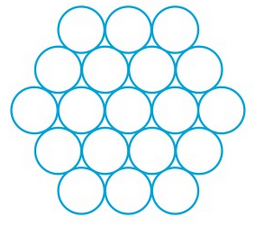
\includegraphics[height=4cm]{./img/lecture20-fig3.png}
    \end{center}
    The figure shows how 19 circles fit into a hexagonal shape with 3 circles
      on each edge. Let $H(n)$ be the number of circles you need to form a hexagon with
      $n$ circles on each edge. From the figure it is clear that $H(2)=7$
       and $H(3)=19$. Find a recurrence relation for $H(n)$.
       
\end{frame}

\begin{frame}[plain]{}

 Answer:
  \[ 
          H(n) = \left\{ \begin{array}{ccc}
                          7 &\mbox{if}& n=2\ \\
                          H(n-1) + 6n - 6&\mbox{if}& n\geq 3.
                         \end{array}
                  \right.             
     \]
 \end{frame}

\end{document}
%%%%%%%%%%%%%%%%%%%%%%%%%%%%%


 
 %\begin{frame}[plain]{}
 
 % {\bf Example 23.3.} Call a binary tree \Blue{complete} if every leaf has depth $n$ and 
 % every nonleaf node has two children (edges). Let $T$ be a complete binary tree of height $n$.
 % Find a recurrence relation $V(n)$ for the number of nodes in $T$. %Essential, sec 3.1.3
 %  \begin{center}
   %     \includegraphics[height=1.5cm]{lecture23-fig6.png}
 %     \end{center}
 % \medskip
 % \pause
  
 % % {\bf Soluton.} The recurrence relation $V(n)$ for the number of nodes in $T$ is 
 %   \[ V(n) = \left\{ \begin{array}{ccc}
 %                      1 &\mbox{if}& n=0\\
 %                      2V(n-1)+1 &\mbox{if} & n>0
 %                     \end{array}\right. 
 %    \]                 
 %  \vspace{1.5in}
   
%\end{frame}



%%%%%%%%%%%%%%%%%%%%%

\begin{frame}[plain]{Exercises}
 \begin{enumerate}

  \item Give a recurrence relation that describes the sequence 3, 6, 12, 24, 48, 96, 192, …
  %Essential, sec 3.1, p162, 20
  
    \item  At the beginning of each day, Andrew adds one gallon of water to his bird bath.
  Each day, one-third of the water in the bird bath evaporates. At the end of day 0, 
  the bird bath contains 8 gallons of water.
  Give a recurrence relation for $W(n)$, the amount of water in the bird bath at the end of day $n$.

      \item Use the reduction formula 
   \[ \int x^ne^x\,dx = x^ne^x - n \int x^{n-1}e^x\,dx \]
    to give a recurrence relation  for
    \[ I(n) = \int_0^1 x^ne^x\,dx \]
    when $n\geq 0$.
     
 \end{enumerate}

\end{frame}

\begin{frame}[plain]{ }
 \begin{enumerate}
   \setcounter{enumi}{3}
 
  \item Suppose that you are collecting coins to make hexagons in a natural way
    by packing circles as tightly as possible.
    \begin{center}
     \includegraphics[height=4cm]{lecture23-fig7.png}
    \end{center}
    The figure shows how 19 circles fit into a hexagonal shape with 3 circles
      on each edge. Let $H(n)$ be the number of circles you need to form a hexagon with
      $n$ circles on each edge. From the figure it is clear that $H(2)=7$
       and $H(3)=19$. Find a recurrence relation for $H(n)$.
 \end{enumerate}

\end{frame}



\begin{frame}[plain]{ }
 \begin{enumerate}
  \setcounter{enumi}{3}
    
      \item Ahmed lends money at outrageous rates of interest. He demands to be paid
     10\% interest \emph{per week} on a loan, compounded weekly.
     Suppose you borrow 500 Dhs from him. Let $M(n)$ = the money you owed at $n$-th week.
     \begin{itemize}
       \item[(a)]  Find the recurrence relation for $M(n)$. 
       \item[(b)] If you wait four weeks to pay him back, how much will you owe?
     \end{itemize}
 
 \end{enumerate}

\end{frame}


 
\begin{frame}[plain]{Iterative Python Code for  Fibonacci Numbers}
 \begin{itemize}
   \item  The \Blue{Fibonacci numbers:} 1, 1, 2, 3, 5, 8, 13, 21, 34, 55, 89, ...  
        \begin{center}
	      \includegraphics[height=3.7cm]{../Lecture_F16/lecture15-fig5.png}
	  \end{center} 
 \end{itemize}

\end{frame}

\begin{frame}[plain]{Recursive Python Code for  Fibonacci Numbers}
 \begin{itemize}
   \item  The \Blue{Fibonacci numbers} $F(n)$ satisfy the following recurrence relation:
     \[ \Blue{
          F(n) = \left\{ \begin{array}{ccc}
                          1 &\mbox{if}& n=1\ \mbox{or}\ n=2\\
                          F(n-1)+F(n-2)&\mbox{if}& n>2.
                         \end{array}
                  \right. 
              }
     \]
        \begin{center}
	      \includegraphics[height=4cm]{../Lecture_F16/lecture15-fig6.png}
	  \end{center} 
 \end{itemize}

\end{frame}


